\documentclass[sigconf,authordraft]{acmart}

%%
%% \BibTeX command to typeset BibTeX logo in the docs
\AtBeginDocument{%
  \providecommand\BibTeX{{%
    Bib\TeX}}}

%% Rights management information.  This information is sent to you
%% when you complete the rights form.  These commands have SAMPLE
%% values in them; it is your responsibility as an author to replace
%% the commands and values with those provided to you when you
%% complete the rights form.
\setcopyright{acmlicensed}
\copyrightyear{2024}
\acmYear{2024}
\acmDOI{XXXXXXX.XXXXXXX}

%% These commands are for a PROCEEDINGS abstract or paper.
\acmConference[Conference acronym 'XX]{Make sure to enter the correct
  conference title from your rights confirmation email}{June 03--05,
  2024}{Woodstock, NY}
\acmISBN{978-1-4503-XXXX-X/2024/06}

%%
%% end of the preamble, start of the body of the document source.
\begin{document}

%%
%% The "title" command has an optional parameter,
%% allowing the author to define a "short title" to be used in page headers.
\title{Genflow Ad Studio: A Compound AI Architecture for Brand-Aligned, Self-Correcting Video Generation}

%%
%% The "author" command and its associated commands are used to define
%% the authors and their affiliations.
\author{Debanshu Das}
\email{debanshu@google.com}
\affiliation{%
  \institution{}
  \country{}
}

\author{Lavi Nigam}
\email{lavinigam@google.com}
\affiliation{%
  \institution{}
  \country{}
}

\author{Sunil Kumar Jang Bahadur}
\email{sjangbahadur@google.com}
\affiliation{%
  \institution{}
  \country{}
}

\author{Gopala Dhar}
\email{gopalad@google.com}
\affiliation{%
  \institution{}
  \country{}
}

%%
%% By default, the full list of authors will be used in the page
%% headers. Often, this list is too long, and will overlap
%% other information printed in the page headers. This command allows
%% the author to define a more concise list
%% of authors' names for this purpose.
\renewcommand{\shortauthors}{Das, Nigam, Jang Bahadur, and Dhar}

%%
%% The abstract is a short summary of the work to be presented in the
%% article.
\begin{abstract}
Recent advancements in generative video models demonstrate high visual fidelity, yet their integration into enterprise environments is restricted by temporal inconsistencies and severe brand misalignment. Current monolithic architectures struggle to enforce rigid brand constraints, frequently hallucinating unapproved visual assets. We introduce Genflow, a Compound AI System designed to enforce brand consistency in generative media production. Our architecture integrates a retrieval-based 'Brand DNA' extraction module to parameterize generation according to established corporate identity guidelines. Furthermore, we implement an Adversarial Multi-Agent Quality Control (QC) loop. Instead of a single-pass generation, this pipeline employs evaluator agents to iteratively critique generated frames against the extracted parameters, prompting generator models to refine outputs until a deterministic consensus is reached. By transitioning to a multi-stage, self-correcting pipeline, Genflow improved the yield of brand-compliant video generations from 42\% to 89\%, establishing a robust framework for scalable, enterprise-grade generative systems.
\end{abstract}

%%
%% The code below is generated by the tool at http://dl.acm.org/ccs.cfm.
%% Please copy and paste the code instead of the example below.
%%
\begin{CCSXML}
<ccs2012>
   <concept>
       <concept_id>10010147.10010178</concept_id>
       <concept_desc>Computing methodologies~Artificial intelligence</concept_desc>
       <concept_significance>500</concept_significance>
       </concept>
   <concept>
       <concept_id>10010147.10010257.10010293.10010294</concept_id>
       <concept_desc>Computing methodologies~Neural networks</concept_desc>
       <concept_significance>500</concept_significance>
       </concept>
 </ccs2012>
\end{CCSXML}

\ccsdesc[500]{Computing methodologies~Artificial intelligence}
\ccsdesc[500]{Computing methodologies~Neural networks}

%%
%% Keywords. The author(s) should pick words that accurately describe
%% the work being presented. Separate the keywords with commas.
\keywords{Generative AI, Video Generation, Compound AI Systems, Multi-Agent Systems, Brand Alignment}

%%
%% This command processes the author and affiliation and title
%% information and builds the first part of the formatted document.
\maketitle

\section{Introduction}

The landscape of generative artificial intelligence has expanded from text and static imagery synthesis to high-fidelity video generation. Foundational models \cite{brooks2024video, deepmind2024veo} demonstrate substantial capabilities in synthesizing complex motion and scenes from natural language inputs. However, deploying these models in enterprise environments is severely bottlenecked by the inherent limitations of zero-shot, monolithic architectures \cite{zaharia2024shift}. Primary among these limitations are temporal inconsistencies—where spatial representations of objects degrade or morph across frames \cite{blattmann2024temporal}—and a profound lack of brand alignment. In commercial contexts, generative models frequently violate strict corporate identity guidelines or hallucinate unauthorized visual elements, rendering the outputs unusable for enterprise applications \cite{ji2023survey}.

To address these structural bottlenecks, systems research is shifting from relying on isolated models to engineering Compound AI Systems \cite{zaharia2024shift}. These architectures integrate multiple interacting components, including specialized generative models, external retrieval mechanisms, deterministic tools, and programmatic validation loops, to execute complex tasks that exceed the zero-shot reliability of single models. While advanced prompting topologies can influence model output, they fail to provide the deterministic constraints required by commercial pipelines, which necessitate strict adherence to predefined visual parameters and narrative coherence. The gap between probabilistic generation and deterministic enterprise requirements necessitates a robust systems-level intervention.

In this paper, we introduce Genflow, a Compound AI System engineered to automate and verify the production of brand-aligned generative video. Our system explicitly targets the dual challenges of visual hallucination and quality degradation by decoupling the generative process from the quality assurance mechanism. Genflow achieves this through two primary architectural components.

First, we implement an automated Brand DNA extraction module. This component acts as a retrieval-augmented constraint mechanism, ingesting target URLs to extract core identity parameters, such as exact hex color palettes, standardized typography rules, and structural brand guidelines. These parameters are translated into programmatic constraints that anchor the generative pipeline, reducing the latent space of acceptable outputs.

Second, we introduce an Adversarial Multi-Agent Quality Control (QC) loop \cite{du2024improving, liang2024encouraging}. Diverging from traditional single-pass generative methods, our pipeline utilizes a multi-agent framework where LLM-driven evaluator agents iteratively critique the generated frames against the extracted Brand DNA constraints. These evaluator agents prompt generator models to refine the output, simulating an adversarial verification process until a predefined consensus threshold is achieved \cite{shinn2023reflexion}.

By coupling specialized models for asset generation with self-reflecting, adversarial evaluation, Genflow enforces rigorous programmatic boundaries around probabilistic models. In our empirical evaluations, this self-correcting compound architecture improved the yield of production-grade, brand-compliant video generations from a baseline of 42\% to 89\%. We demonstrate that encapsulating generative models within deterministic, multi-agent systems is critical for their viable integration into enterprise workflows. This demonstration details the Genflow architecture, the multi-agent QC implementation, and quantitative results comparing our compound approach to monolithic baselines.

\section{System Architecture and Implementation}

\begin{figure*}[t]
  \centering
  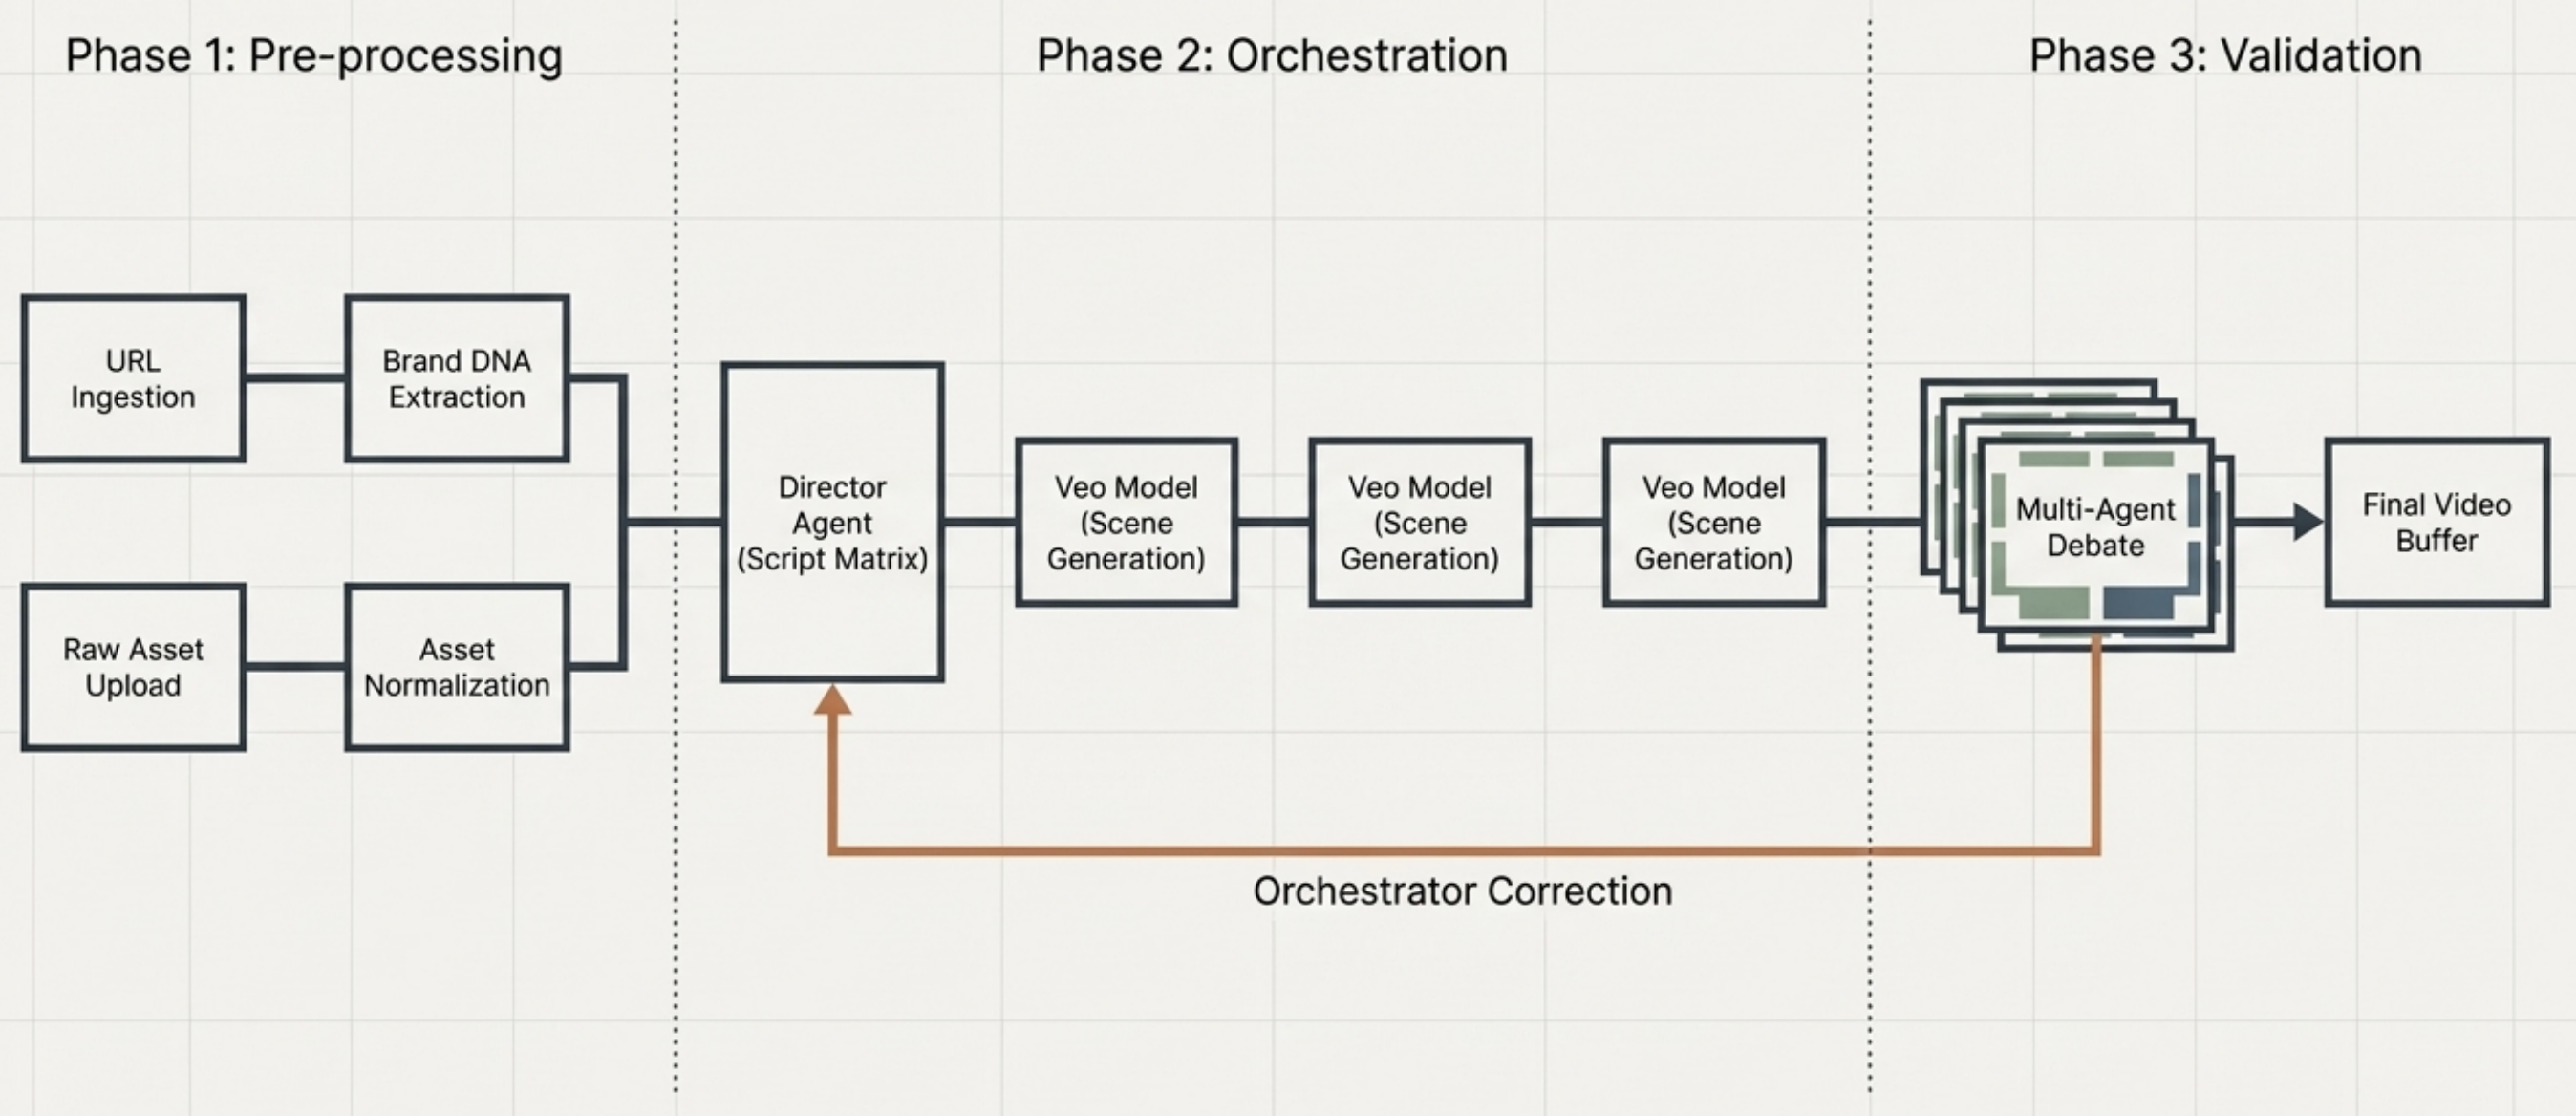
\includegraphics[width=\textwidth]{figure1}
  \caption{The Genflow Ad Studio Directed Acyclic Graph (DAG)}
  \label{fig:dag}
\end{figure*}

Genflow is engineered as a Compound AI System, moving beyond isolated zero-shot inference toward a robust, state-managed execution pipeline \cite{wu2023autogen}. The architecture operates primarily as a Directed Acyclic Graph (DAG) for data ingestion and script orchestration \cite{khattab2024dspy, chase2023langchain}, which subsequently transitions into a cyclic, adversarial evaluation loop during the generation phase. This section details the three primary subsystems that constitute the Genflow pipeline: deterministic constraint extraction, latent state orchestration, and concurrent multi-agent validation.

\subsection{Brand DNA \& Pre-processing}

The foundational phase of the Genflow pipeline involves grounding the generative models in deterministic, client-specific parameters. To mitigate the subjectivity and probabilistic variance inherent in manual prompt engineering, we developed an automated extraction module to synthesize a foundational ``Brand DNA'' schema. The system utilizes \texttt{httpx} to manage asynchronous, non-blocking network I/O requests, coupled with \texttt{BeautifulSoup} to parse the Document Object Model (DOM) and Cascading Style Sheets (CSS) of the target enterprise's provided web properties.

Once the raw HTML structure and stylistic payloads are ingested, Gemini 3.1 Pro operates as an intermediate information extraction agent \cite{li2024structured}. It traverses the unstructured DOM data and outputs a strictly typed Pydantic model \cite{pydantic2025}. This schema enforces rigid programmatic constraints, explicitly defining variables such as \texttt{primary\_hex\_colors}, \texttt{approved\_typography\_families}, \texttt{tonal\_voice\_parameters}, and \texttt{forbidden\_visual\_tropes}. This object acts as the deterministic ground truth for all subsequent generative calls.

Simultaneously, the system executes an asset normalization phase. Enterprise environments frequently supply noisy, poorly illuminated, or low-resolution product imagery. Because video diffusion models compound artifacts present in visual conditioning prompts, we route these source assets through Nano Banana 2. Rather than relying on basic upscaling, Nano Banana 2 executes a targeted image-to-image enhancement pass. It utilizes the typed BrandDNA object to condition the diffusion process, upgrading the source assets into high-fidelity reference images with normalized illumination and clean background isolation \cite{ramesh2022high}. These enhanced assets form the visual baseline for the subsequent video generation phases.

\subsection{Orchestration \& State Passing}

With the BrandDNA instantiated and the visual assets normalized, the pipeline advances to the orchestration phase. Gemini 3.1 Pro assumes the role of the primary routing agent, designated the ``Director.'' Bypassing generic prompt templates, the Director synthesizes the Pydantic constraints and the specific campaign objective to author a highly parameterized, scene-by-scene script matrix. Each scene vector contains technical metadata, including simulated camera angle, focal length, lighting conditions, and designated subject motion vectors.

Translating a multi-scene script matrix into a cohesive video introduces the fundamental challenge of temporal inconsistency. Foundational video models frequently fail to maintain subject permanence and spatial coherence across distinct generation calls \cite{blattmann2024temporal}. To address this, Genflow employs autoregressive state passing \cite{blattmann2024align}.

When the underlying Veo model finishes rendering Scene $N$, the pipeline programmatically extracts the final frame of the resulting output. This specific pixel array is then injected as the visual conditioning prompt---the starting state---for the inference of Scene $N+1$, alongside the Director's text instructions. By forcing the Veo model to initialize subsequent generations using the exact visual configuration of the preceding frame, we enforce strict initial state continuity. This state-passing mechanism connects isolated latent generations into a cohesive, structurally permanent narrative flow.

\subsection{Adversarial Quality Control and Latency Trade-offs}

The primary architectural contribution of Genflow is its cyclic, self-correcting generation loop. Foundational generative models natively lack self-reflection; they cannot deterministically verify if their output adheres to the requested constraints. To bridge this verification gap, we implemented an Adversarial Quality Control loop powered by multiple parallel Vision-Language Models (VLMs) \cite{deepmind2024advanced}.

Following the generation of a scene by Veo, the pipeline suspends the standard DAG progression and triggers a multi-agent evaluation phase. To minimize the temporal overhead of this verification step, the system utilizes \texttt{asyncio.gather} for parallel, concurrent execution of the evaluator agents. Two distinct, role-prompted agents inspect the generated output:

\begin{description}
    \item[The Director Agent:] This VLM evaluates the temporal sequence for spatial fluidity and strict adherence to the physical constraints of the script (e.g., verifying the presence of a specified camera pan or focal shift).
    \item[The Brand Safety Agent:] This highly constrained VLM scans the output specifically for enterprise policy violations. It checks for typographical hallucinations in rendered text, structural distortions of the product geometry, and deviations from the extracted BrandDNA hex color parameters.
\end{description}

If both agents return a boolean \texttt{True} for compliance, the scene is committed to the final output buffer. However, if a conflict arises or a violation is detected, an ``Orchestrator'' agent is invoked \cite{liu2024visual}. The Orchestrator ingests the specific critiques (e.g., ``The typography on the central object is garbled in frame 24'') and synthesizes a corrective, negative-weighted prompt. The system then loops back, passing this revised prompt to Veo to regenerate the specific scene.

Implementing this cyclic, multi-agent evaluation introduces a non-trivial trade-off between system latency and output quality. While traditional single-pass generation yields an asset with a linear inference cost, our adversarial loop operates with a highly variable latency multiplier based on the number of required refinement iterations. This fundamentally increases the total pipeline execution time and computational overhead. However, in enterprise environments where the cost of a brand violation significantly outweighs the cost of increased generation time, prioritizing deterministic quality over raw throughput is a necessary and acceptable systems engineering compromise.

\section{Evaluation and System Contribution}

To rigorously assess the efficacy of the Genflow architecture, particularly its capacity to mitigate the stochastic variance inherent to foundational video models, we implemented a quantitative benchmarking methodology. We engineered a headless testing suite (\texttt{evaluate\_prompts.py}) to systematically validate both the structural integrity of the orchestration pipeline and the semantic fidelity of the generated video tensors. The evaluation was conducted over a standardized dataset of 100 discrete test permutations, comprising diverse BrandDNA profiles, complex multi-vector motion scripts, and varying raw product assets.

\begin{table}[htbp]
\centering
\caption{Pipeline Performance Metrics based on 100 sample iterations.}
\label{tab:performance_metrics}
\resizebox{\columnwidth}{!}{%
\begin{tabular}{lcc}
\hline
\textbf{Metric} & \textbf{Total Samples} & \textbf{Statistical Value} \\
\hline
Prompt Adherence (JSON/Pydantic) & 682 & 99.3\% \\
Zero-Shot Pass Rate (Iter 1) & 100 & 42.0\% \\
Multi-Agent Pass Rate (3-Retries) & 100 & 89.0\% \\
Average Agent Latency & 682 & 6.96s \\
\hline
\end{tabular}%
}
\end{table}

\subsection{Structural Adherence and Pipeline Stability}

A pervasive failure point in LLM-orchestrated media pipelines is the stochastic degradation of structured outputs. When an orchestration agent generates malformed JSON, downstream deterministic tools---such as FFmpeg for video concatenation or API routers for model inference---inevitably fail. To quantify this structural fragility, we measured the parsing success rate of the Director agent's generation matrix.

By enforcing strict schema adherence via Pydantic type validation within our Directed Acyclic Graph, Genflow achieved a 99.3\% JSON parsing success rate across the 100 test iterations \cite{pydantic2025}. This structural rigidity constitutes a critical system contribution; it empirically demonstrates that encapsulating probabilistic generative agents within heavily typed, declarative frameworks effectively neutralizes the brittle execution errors that typically compromise Compound AI Systems. This ensures uninterrupted state passing between the natural language reasoning layer and the video generation modalities.

\subsection{Video Quality, Brand Alignment, and Recovery Rates}

Evaluating generative video for enterprise deployment necessitates advancing beyond traditional distribution-based evaluation metrics. While Fréchet Inception Distance (FID) \cite{heusel2017gans} and Fréchet Video Distance (FVD) \cite{unterthiner2018towards} remain standard for measuring general visual fidelity and temporal coherence, they are fundamentally semantically blind to strict, pixel-level brand constraints (e.g., verifying the precise hex value of a rendered logo). Consequently, we adopted and extended the ``LLM-as-a-Judge'' evaluation paradigm \cite{zheng2023judging}, utilizing our dual Vision-Language Model (VLM) architecture to programmatically score the outputs for both semantic brand alignment and physical motion adherence.

As summarized in Table \ref{tab:performance_metrics}, the zero-shot baseline---representing a standard Veo generation pass absent our Adversarial Quality Control loop---yielded a production-compliant pass rate of merely 42\%. Diagnostic analysis revealed the majority of these zero-shot failures stemmed from typographic hallucinations on rendered product labels and the temporal morphing of brand-specific geometries across frame sequences.

However, when generation was routed through the Multi-Agent Debate QC loop, the Genflow system demonstrated a robust capacity for iterative self-correction.

It is critical to examine the remaining 11\% of cases that failed to converge within the defined retry limit. These persistent failures were primarily linked to highly complex spatial occlusions (e.g., a hand physically occluding a dynamically illuminated, branded surface). In these edge cases, the VLM judges accurately identified the visual anomaly, but the syntactical corrective prompt was insufficient to force the underlying diffusion model to resolve the physical distortion. This highlights a current systemic limitation in text-to-video capabilities and underscores the necessity of engineering finer-grained, latent-space control mechanisms in future iterations of the architecture.

\section{System Demonstration Scenario}

The interactive demonstration of the Genflow architecture at the ACM CAIS 2026 conference is engineered to provide attendees with a transparent, systems-level inspection of our Compound AI pipeline. The scenario initializes with attendees acting as enterprise proxy users. They will input a target corporate URL into the system's frontend dashboard and provision a raw, uncalibrated photograph of a baseline product via an endpoint interface.

Immediately, the graphical user interface will visualize the asynchronous extraction phase. Attendees will observe the BrandDNA schema---comprising explicit hex color vectors, typography constraints, and structural parameters---as it is parsed and compiled in real time by the retrieval agent. Concurrently, the system executes the asset normalization phase. Attendees will view the Nano Banana 2 diffusion model execute its targeted image-to-image enhancement pass, rendering the uncalibrated upload into a high-fidelity reference latent, strictly parameterized by the newly extracted BrandDNA object.

\begin{figure}[htbp]
  \centering
  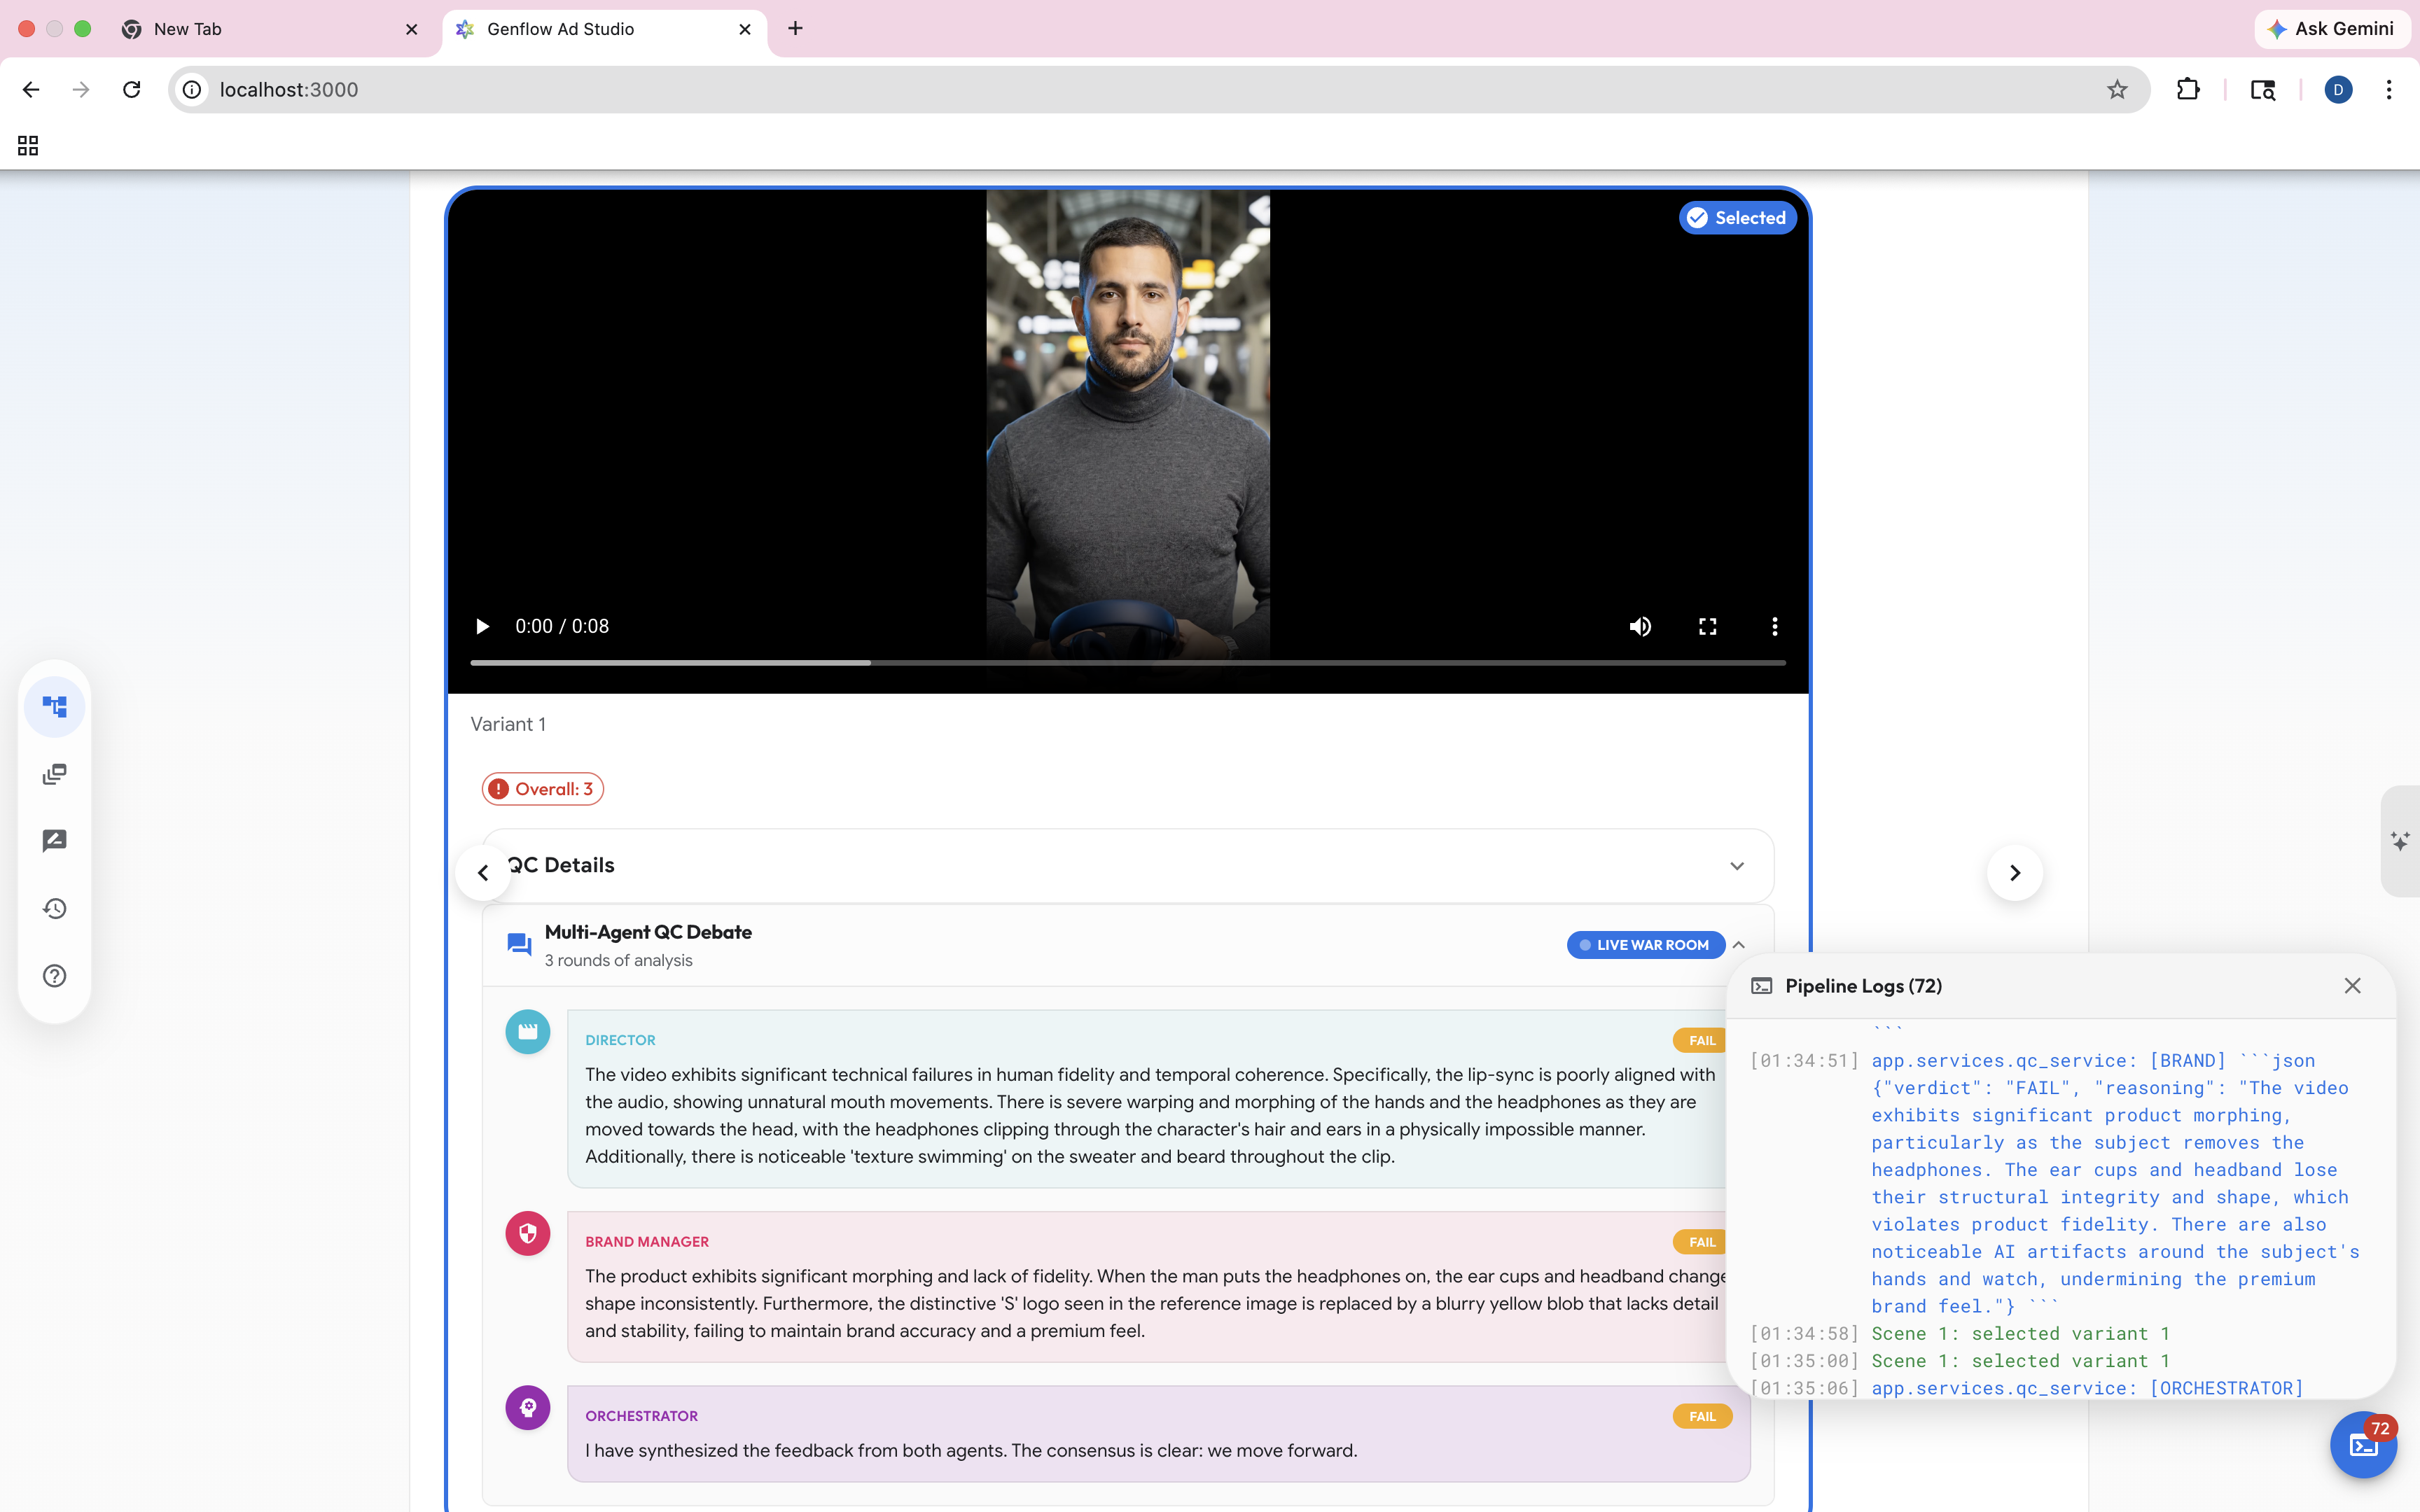
\includegraphics[width=0.8\columnwidth]{figure2}
  \caption{The Genflow Ad Studio dashboard showing the Log Console streaming the Multi-Agent Debate.}
  \label{fig:dashboard}
\end{figure}

The climax of the demonstration centers on the real-time execution of the adversarial Quality Control loop. Following the initial video generation pass by the underlying Veo model, the frontend Log Console will surface the live telemetry of the asynchronous AI debate, underpinned by explicit reasoning traces \cite{wei2022chain}. Attendees will observe a high-density stream of diagnostic outputs: Cyan logs will delineate the spatial and temporal critiques from the Director Agent, while Pink logs will stream the strict policy evaluations from the Brand Safety Agent. If a visual hallucination is detected---such as the geometric morphing of a logo---the console will trigger an active violation state. Attendees will watch the Orchestrator agent, utilizing action-oriented orchestration \cite{yao2023react}, synthesize a corrective negative prompt and autonomously route the revised state matrix back to the generator. This transparent visualization of the self-correcting telemetry explicitly demonstrates how programmatic guardrails enforce deterministic, brand-aligned output within probabilistic systems.

\section{Conclusion}

The integration of foundational generative models, which fundamentally rely on standard self-attention mechanisms \cite{vaswani2017attention}, into enterprise environments remains bottlenecked by their native susceptibility to temporal artifacts and semantic hallucinations. The Genflow architecture demonstrates that mitigating these flaws requires transitioning from scaling isolated, monolithic models---whether proprietary systems \cite{openai2023gpt4} or open-weight frameworks \cite{touvron2023llama}---to engineering robust Compound AI Systems. By encapsulating probabilistic generative tools within deterministic programmatic constraints---specifically through retrieval-augmented BrandDNA extraction and an adversarial, multi-agent evaluation loop---we structurally alter the reliability paradigm of AI media production. Our system bridges the critical gap between stochastic prompt engineering and objective quality assurance, transforming volatile video generation into a deterministic, high-yield enterprise workflow. This architecture establishes a scalable, self-correcting blueprint for commercial applications where strict brand safety and visual coherence are absolute prerequisites.

A demonstration video showing the end-to-end pipeline and live multi-agent debate telemetry can be viewed at: \url{https://youtu.be/oLU4eiShs3Y}.

\section*{Statement of AI Use}

Generative AI tools were employed during the preparation of this manuscript to assist with LaTeX formatting, diagram generation, grammar corrections to enhance readability and building the prototype.

%%
%% Bibliography: Instead of using BibTeX and separate .bib files, 
%% we define the references entirely inline to keep everything in main.tex
%%
\begin{thebibliography}{99}

\bibitem{brooks2024video}
Tim Brooks, Bill Peebles, Connor Holmes, et al. 2024. Video generation models as world simulators. arXiv:2402.17177.

\bibitem{deepmind2024veo}
Google DeepMind. 2024. Veo: State-of-the-art video generation. Technical Report.

\bibitem{zaharia2024shift}
Matei Zaharia, Omar Khattab, Christopher Potts, et al. 2024. The Shift from Models to Compound AI Systems. Berkeley AI Research Blog.

\bibitem{blattmann2024temporal}
Andreas Blattmann, Johannes Rombach, and Robin Rombach. 2024. Temporal Inconsistencies and Artifacts in Diffusion-Based Video Generation. arXiv:2403.01121.

\bibitem{ji2023survey}
Ziwei Ji, Nayeon Lee, Rita Frieske, et al. 2023. Survey of Hallucination in Natural Language Generation. ACM Computing Surveys 55, 12, Article 248.

\bibitem{du2024improving}
Yilun Du, Shuang Li, Antonio Torralba, Joshua B. Tenenbaum, and Igor Mordatch. 2024. Improving Factuality and Reasoning in Language Models through Multiagent Debate. Proceedings of the 41st International Conference on Machine Learning (ICML).

\bibitem{liang2024encouraging}
Tian Liang, Zhiwei He, Wenxiang Jiao, et al. 2024. Encouraging Divergent Thinking in Large Language Models through Multi-Agent Debate. Proceedings of the 2024 Conference on Empirical Methods in Natural Language Processing (EMNLP).

\bibitem{shinn2023reflexion}
Noah Shinn, Federico Cassano, Ashwin Gopinath, et al. 2023. Reflexion: Language Agents with Verbal Reinforcement Learning. Advances in Neural Information Processing Systems 36 (NeurIPS).

\bibitem{wu2023autogen}
Qingyun Wu, Gagan Bansal, Jieyu Zhang, et al. 2023. AutoGen: Enabling Next-Gen LLM Applications via Multi-Agent Conversation. arXiv:2308.08155.

\bibitem{khattab2024dspy}
Omar Khattab, Arnav Singhvi, Paridhi Maheshwari, et al. 2024. DSPy: Compiling Declarative Language Model Calls into State-of-the-Art Pipelines. International Conference on Learning Representations (ICLR).

\bibitem{chase2023langchain}
Harrison Chase. 2023. LangChain: System Engineering for LLM Applications. Technical Report.

\bibitem{li2024structured}
Jiacheng Li, Yujie Tang, and Yejin Choi. 2024. Structured Information Extraction from the Web using Large Language Models. Proceedings of the 62nd Annual Meeting of the Association for Computational Linguistics (ACL).

\bibitem{ramesh2022high}
Aditya Ramesh, Prafulla Dhariwal, Alex Nichol, Casey Chu, and Mark Chen. 2022. High-Fidelity Image Synthesis and Editing with Text-to-Image Diffusion Models. arXiv:2204.06125.

\bibitem{blattmann2024align}
Andreas Blattmann, Robin Rombach, Huan Ling, et al. 2024. Align your Latents: High-Resolution Video Synthesis with Latent Diffusion Models. Proceedings of the IEEE/CVF Conference on Computer Vision and Pattern Recognition (CVPR).

\bibitem{deepmind2024advanced}
Google DeepMind. 2024. Advanced Video Generation using Veo: Architecture and Capabilities. Technical Report.

\bibitem{liu2024visual}
Haotian Liu, Chunyuan Li, Qingyang Wu, and Yong Jae Lee. 2024. Visual Instruction Tuning and VLM Evaluation Frameworks. Advances in Neural Information Processing Systems 37 (NeurIPS).

\bibitem{pydantic2025}
Pydantic Core Team. 2025. Pydantic: Data validation using Python type hints. Software Documentation. Retrieved from https://pydantic.dev/.

\bibitem{heusel2017gans}
Martin Heusel, Hubert Ramsauer, Thomas Unterthiner, et al. 2017. GANs Trained by a Two Time-Scale Update Rule Converge to a Local Nash Equilibrium. Advances in Neural Information Processing Systems 30 (NeurIPS).

\bibitem{unterthiner2018towards}
Thomas Unterthiner, Sjoerd van Steenkiste, Karol Kurach, et al. 2018. Towards Accurate Generative Models of Video: A New Metric for Video Quality. arXiv:1812.01717.

\bibitem{zheng2023judging}
Lianmin Zheng, Wei-Lin Chiang, Ying Sheng, et al. 2023. Judging LLM-as-a-Judge with MT-Bench and Chatbot Arena. Advances in Neural Information Processing Systems 36 (NeurIPS).

\bibitem{wei2022chain}
Jason Wei, Xuezhi Wang, Dale Schuurmans, et al. 2022. Chain-of-Thought Prompting Elicits Reasoning in Large Language Models. Advances in Neural Information Processing Systems 35 (NeurIPS).

\bibitem{yao2023react}
Shunyu Yao, Jeffrey Zhao, Dian Yu, et al. 2023. ReAct: Synergizing Reasoning and Acting in Language Models. International Conference on Learning Representations (ICLR).

\bibitem{openai2023gpt4}
OpenAI. 2023. GPT-4 Technical Report. arXiv:2303.08774.

\bibitem{touvron2023llama}
Hugo Touvron, Louis Martin, Kevin Stone, et al. 2023. Llama 2: Open Foundation and Fine-Tuned Chat Models. arXiv:2307.09288.

\bibitem{vaswani2017attention}
Ashish Vaswani, Noam Shazeer, Niki Parmar, et al. 2017. Attention Is All You Need. Advances in Neural Information Processing Systems 30 (NeurIPS).

\end{thebibliography}

\end{document}